Un pedal de efectos es un dispositivo que se conecta entre un instrumento (normalmente electrófono) y su amplificador encargándose de modificar la señal de entrada y sus características fundamentales como pueden ser timbre, tono y volumen. En este proyecto se pretende estudiar las posibilidades de diseño e implementación de uno de estos pedales, enfocándolo a un uso con instrumentos de viento, en concreto el saxofón puesto que es el instrumento que yo toco. Generalmente, no es habitual el uso de pedales de efectos en instrumentos de viento, ya que en general se busca mantener el sonido lo más fiel posible al producido por el instrumento. No obstante, en multitud de producciones se pueden apreciar efectos añadidos en postproducción ya sea digital o analógicamente. Algunos ejemplos son el \emph{reverb} o el \emph{chorus}. Sin embargo, aqui se pretende implementar un efecto de octavador, el cual se describirá posteriormente.

Se ha decidido el combinar este efecto con la implementación en formato de pedal. Este formato se ha hecho muy popular desde su aparición, debido a que los intérpretes pueden activarlo con el pie pudiendo mantaner las manos en el instrumento. Aunque los intérpretes de instrumentos de viento no están acostumbrados al uso de pedales, se mantiene la idea del pedal por analogía con otros instrumentos.

Este proyecto abarca todo el proceso desde la idea inicial, diseño y montaje del prototipo final, por tanto, las especificaciones de funcionamiento que se han utilizado pretenden facilitar un uso profesional del prototipo, de forma que sea compatible con los estándares establecidos en el contexto musical e ingenieril al mismo tiempo.

El flujo de datos será el siguiente. En primer lugar se utiliza un transductor para adquirir la señal, en este caso, un micrófono convencional. Una vez que el estímulo externo es transformado en pulsos eléctricos, atravesará un etapa de entrada analógica que pre-amplifica la señal y la adecúa a la entrada de la FPGA.

Para el prototipo se ha utilizado la placa proporcionada por el departamento: Nexys A7. Esta placa monta una FPGA \emph{Xilinx XC7A100T-1CSG324C} junto con varios switches, botones, leds y displays de 7 segmentos, que harán más fácil el manejo de la misma. Esta placa tiene un micrófono integrado, pero es de tan baja calidad que se opta por diseñar la etapa de entrada, analógica completamente, y conectarla con uno de los puertos del \emph{Pmod i2s2}, también de Digilent y proporcionado por el departamento. Este módulo contiene ADC, DAC y los conectores de mini-jack estándar en formato de audio, que servirán para gestionar la señal de entrada y la de salida.

Se implementará un algoritmo que se encargará de llevar a cabo la octavación de la señal de entrada y de proporcionarla en la salida. Este algoritmo utiliza una aproximación de \emph{Phase Vocoder} muy común en el tratamiento de señales de audio realizando una transformación al dominio de la frecuencia mediante FFT. Durante todo el proceso se priorizará el criterio de la baja latencia, dado que si no, resulta imposible operar en tiempo real. El algoritmo se describirá en profundidad en su capítulo correspondiente.

\section{Objetivos}
Para la realización de este proyecto de forma satisfactoria se ha establecido la consecución de una serie de objetivos que son los siguientes:
\begin{itemize}
\item Diseño de un sistema completo, a partir de una problemática definida previamente mediante el estudio del instrumento y las señales.
\item Implementación sobre la FPGA proporcionada.
\item Construcción de un prototipo para estudiar la problemática desde la práctica.
\item Afianzar, debido a todo esto, conocimientos adquiridos durante el Grado en diversos ámbitos como el procesamiento de señal y en concreto en la especialidad de Sistemas Electrónicos como la programación hardware, el montaje de un circuito analógico y la correcta comunicación entre todos los módulos.
\end{itemize}

\section{Metodología}
\begin{itemize}
\item En primer lugar se seleccionará el efecto que se quieren implementar, dando prioridad al octavador.
\item Como segundo paso, se estudiará la literatura existente y se probarán distintas soluciones algorítmicas empleando MATLAB.
\item Estudio y elección de la interfaces de entrada y salida. Selección de micrófono, ADC y DAC.
\item Desarrollo y verificación en VHDL empleando la herramienta VIVADO de Xillinx.
\item Montaje de un prototipo empleando la placa Nexys A7 de Digilent, el micrófono seleccionado anteriormente y el resto de dispositivos que fueran necesarios.
\item Test y depuración.
\end{itemize}

\section{Fundamentos del sonido y teoría musical}
Considero necesario hacer un pequeña introducción a algunos conceptos que tendrán importancia para el desarrollo del tranajo en relación con la física del sonido y la teoría musical, para facilitar la comprensión del documento por un público no especializado en estos ámbitos. 
En primer lugar cabe destacar que como cualquier fenómeno físico, un sonido lleva asociados una serie de parámetros matemáticos que lo definen, pero tradicionalmente, estos términos han recibido otro nombre en el ámbito musical, con el que se enseñan en escuelas y conservatorios. Es importante, por tanto, tener clara la relación entre la nomenclatura musical y la equivalencia física y matemática.
\begin{itemize}
\item \textbf{Tono:} hace referencia a la altura de la nota en cuanto a grave o aguda. En parámetro que la define es la frecuencia, que se mide en $Hz$. Aunque el oído humano puede llegar a percibir señales de hasta 20kHz, las notas fundamentales rara vez sobrepasan los 2kHz.
\item \textbf{Volumen:} equivale a la intensidad que posee la señal tanto eléctricamente como cuando se propaga por el aire como una onda de presión. Cuando se mide en un circuito eléctrico se utilizan unidades de tensión mientras que como onda se suelen utilizar los dB dado su carácter logarítmico, sin embargo, posee unidades de intensidad acústica: $W/m^{2}$.
\item\textbf{Timbre:} es característico de cada fuente de sonido y es lo que nos permite diferenciar un instrumento de otro, o voces humanas entre si, aún produciendo la misma nota.
\end{itemize}

La lista de aqui arriba muestra los tres parámetros fundamentales de un sonido musical, sin embargo, no queda claro como funciona el mecanismo matemático que rige el funcionamiento del timbre.

\subsection{Timbre, armónicos y serie armónica}
Cualquier estudiente de ingeniería ha estudiado la generación de armónicos en el contexto de la física y las vibraciones. Sin embargo, puede que no tantos se hayan preguntado como se \emph{oyen} estos modos o si se pueden percibir. La respuesta es sí, y además con mucha claridad. En lo que se refiere a la música, tanto los instrumentos musicales como la voz humana son estructuras complejas que producen sonidos a muchas frecuencias diferentes al mismo tiempo. Nuestro cerebro, cuando oye un sonido se encarga de interpretar la señal recibida para producir un sonido identificable. 

Es inevitable establecer una analogía entre este funcionamiento y el terorema de Fourier, que dice que podemos descomponer cualquier señal como suma de una o varias componentes sinusoidales. Esta poderosa afirmación explica como funciona la generación de cualquier sonido musical.

Así pues, cuando se produce una nota con un instrumento, se generan varias vibraciones a distintas frecuencias, en consecuencia, es la relación entre estas componentes lo que modifica el timbre de la nota generada y nos permite identificarla. La trampa está en que las frecuencias que se producen no son aleatorias, son una serie de notas que reciben el nombre de \emph{armónicos}. El conjunto de estos armónicos se llama \emph{serie armónica}.

\begin{figure}[!ht]
\begin{center}
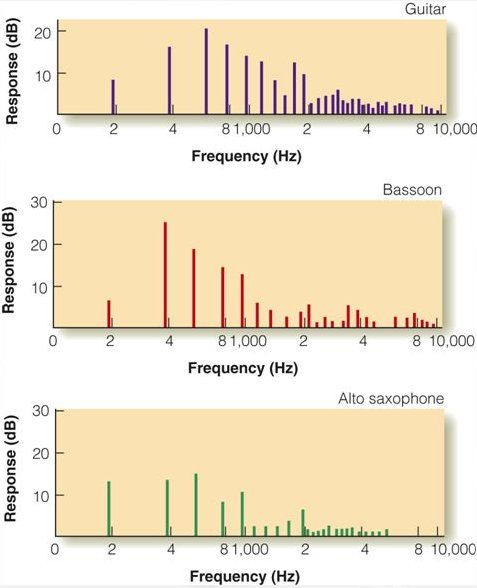
\includegraphics[width=10cm]{img/armonicos.jpg}
\caption{\label{fig:armonicos}Diferentes instrumentos interpretando una misma nota}
\end{center}
\end{figure}


Así pues, podemos concluir con que cada nota está a su vez formada por varios armónicos presentándose en diferente proporción entre ellos. El armónico que define el sonido es el primero de la serie y recibe el nombre de fundamental, el resto se obtienen multiplicando esta frecuencia por números enteros. En la imagen \ref{fig:armonicos} vemos como una guitarra, un fagot y un saxofón generan una mezcla de armónicos diferentes cuando interpretan la misma nota. Las operaciones que vamos realizar en la señal de entrada tienen como objetivo modificar el tono de una nota introducida mientras mantenemos inalterados su volumen y su timbre. En la práctica veremos como tanto el algoritmo como la FPGA introducen desviaciones y no idealidades que nos permiten elaborar y clasificar diferentes métodos y operativas.